
\subsection{Multipole Graph Neural Operator (MGNO)}
\label{sec:multipole}
A natural extension to directly working with kernels in a tensor product form as in Section~\ref{sec:lowrank} is to instead consider kernels that can be well approximated by such a form. This assumption gives rise to the fast multipole method (FMM) which employs a multi-scale decomposition of the kernel in order to achieve linear complexity in computing \eqref{eq:onelayerlinear}; for a detailed discussion see e.g. \citep[Section 3.2]{e2011principles}. FMM can be viewed as a systematic approach to combine the sparse and low-rank approximations to the kernel matrix. Indeed, the kernel matrix is decomposed into different ranges and a hierarchy of low-rank structures is imposed on the long-range components.  We employ this idea to construct hierarchical, multi-scale graphs, without being constrained to particular forms of the kernel.  We will elucidate the workings of the FMM through matrix factorization.
This approach was first outlined in \cite{li2020multipole} and is referred as the Multipole Graph Neural Operator (MGNO).


The key to the fast multipole method's linear complexity lies in the subdivision of the kernel matrix according to the range of interaction, as shown in Figure \ref{fig:hmatrix}: 
\begin{equation}\label{eq:decomposition_matrix}
K = K_1 + K_2 + \ldots + K_L,
\end{equation}
where $K_\ell$ with $\ell=1$ corresponds to the shortest-range interaction, and $\ell=L$  corresponds to the longest-range interaction; more generally index $\ell$ is ordered by the
range of interaction. While the uniform grids depicted in Figure \ref{fig:hmatrix} produce an orthogonal decomposition of the kernel, the decomposition may be generalized to arbitrary discretizations  by allowing slight overlap of the ranges. 


%Notice, when the discretization is a uniform grid, it is possible to have an orthogonal decomposition of the kernel. In general, we allow kernels $K_L$ to overlap with each other. $L$ is the number of levels that usually scales to $O(\log n)$. 

\begin{figure}[h]
    {\centering
    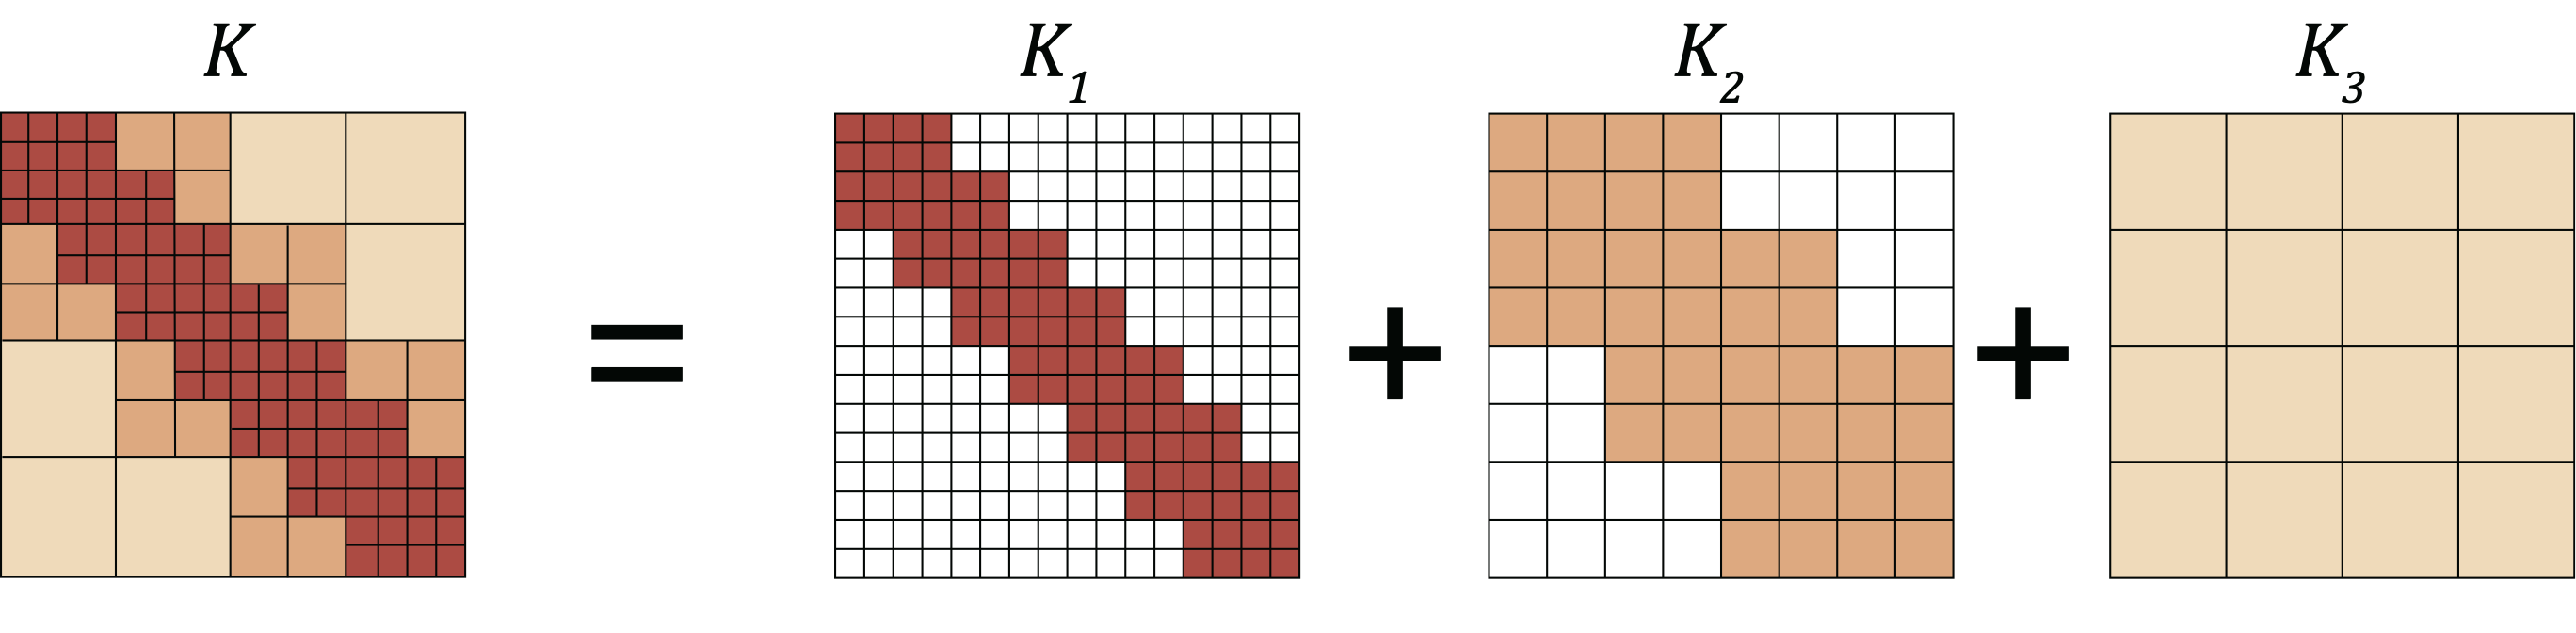
\includegraphics[width=\textwidth]{Figs/Hmatrix.png}
    \caption{Hierarchical matrix decomposition}
    \label{fig:hmatrix}
    \small{
    The kernel matrix $K$ is decomposed with respect to its interaction ranges. $K_1$ corresponds to short-range interaction; it is sparse but full-rank. $K_3$ corresponds to long-range interaction; it is dense but low-rank.
    }
    }
\end{figure}

\paragraph{Multi-scale Discretization.}
We produce a hierarchy of $L$ discretizations with a decreasing number of nodes $J_1 \geq \ldots \geq J_L$ and increasing kernel integration radius $r_1  \leq \ldots \leq r_L$. Therefore, the shortest-range interaction $K_1$ has a fine resolution but is truncated locally, while the longest-range interaction $K_L$ has a coarse resolution, but covers the entire domain. This is shown pictorially in Figure \ref{fig:hmatrix}.
The number of nodes $J_1 \geq \ldots \geq J_L$, and the integration radii $r_1  \leq \ldots \leq r_L$ are hyperparameter choices and can be picked so that the total computational complexity is linear in \(J\). 

A special case of this construction is when the grid is uniform. Then our formulation reduces to the standard fast multipole algorithm and the kernels $K_l$ form an orthogonal decomposition of the full kernel matrix $K$.
Assuming the underlying discretization \(\{x_1,\dots,x_J\} \subset D\) is a uniform grid with resolution $s$ such that $s^d = J$, the $L$ multi-level discretizations will be grids with resolution $s_l = s/2^{l-1}$, and consequentially $J_l = s_l^d = (s/2^{l-1})^d$ . In this case $r_l$ can be chosen as $1/s$ for \(l=1,\dots,L\).
To ensure orthogonality of the discretizations, the fast multipole algorithm sets the integration domains to be $B(x, r_l) \setminus B(x, r_{l-1})$ for each level \(l=2,\dots,L\), so that the discretization on level $l$ does not overlap with the one on level $l-1$. Details of this algorithm can be found in e.g. \citet{greengard1997new}.

\paragraph{Recursive Low-rank Decomposition.}
The coarse discretization representation can be understood as recursively applying an inducing points approximation \citep{quinonero2005aunifying}: starting from a discretization with $J_1 = J$ nodes, we impose inducing points of size $J_2, J_3,\dots, J_L$  which all admit a low-rank kernel matrix decomposition of the form (\ref{eq:nystrom_matrix}). 
The original $J \times J$ kernel matrix $K_l$ is represented by a much smaller $J_l \times J_l$ kernel matrix, denoted by $K_{l,l}$.
As shown in Figure \ref{fig:hmatrix},  $K_1$ is full-rank but very sparse while $K_L$ is dense but low-rank. Such structure can be achieved by applying equation (\ref{eq:nystrom_matrix}) recursively to equation (\ref{eq:decomposition_matrix}), leading to the multi-resolution matrix factorization \citep{kondor2014multiresolution}:
\begin{equation}\label{eq:hierarchy_decomposition}
K \approx K_{1,1} + K_{1,2}K_{2,2}K_{2,1} + K_{1,2}K_{2,3}K_{3,3}K_{3,2}K_{2,1} + \cdots
\end{equation}
where $ K_{1,1} = K_1$ represents the shortest range, $K_{1,2}K_{2,2}K_{2,1} \approx K_2$, represents the  second shortest range, etc. The center matrix $K_{l,l}$ is a $J_l \times J_l$ kernel matrix corresponding to the $l$-level of the discretization described above. The matrices $K_{l+1,l}, K_{l,l+1}$ are  $J_{l+1} \times J_l$ and $J_{l} \times J_{l+1}$  wide and long respectively block transition matrices. 
Denote $v_l \in R^{J_l \times n}$ for the representation of the input \(v\) at each level of the discretization for \(l=1,\dots,L\), and $u_l \in R^{J_l \times n}$ for the output (assuming the inputs and outputs has the same dimension). We define the matrices $K_{l+1,l}, K_{l,l+1}$ as moving the representation \(v_l\) between different levels of the discretization via an integral kernel that we learn. 
Combining with the truncation idea introduced in subsection~\ref{sec:graphneuraloperator}, we define the transition matrices as discretizations of the following integral kernel operators:

\begin{align}
\label{eq:all1}
&K_{l,l}: v_l \mapsto u_{l} = \int_{B(x,r_{l,l})} \kappa_{l,l}(x,y)v_l(y) \: \text{d}y \\ \label{eq:all2}
&K_{l+1,l}: v_l \mapsto u_{l+1} = \int_{B(x,r_{l+1,l})} \kappa_{l+1, l}(x,y)v_l(y) \: \text{d}y \\
\label{eq:all3}
&K_{l, l+1}: v_{l+1} \mapsto u_{l} = \int_{B(x,r_{l,l+1})} \kappa_{l,l+1}(x,y)v_{l+1}(y) \: \text{d}y 
\end{align}
where each kernel \(\kappa_{l,l'} : D \times D \to \R^{n \times n}\) is parameterized as a neural network and learned.

\begin{figure}[t]
    {\centering
    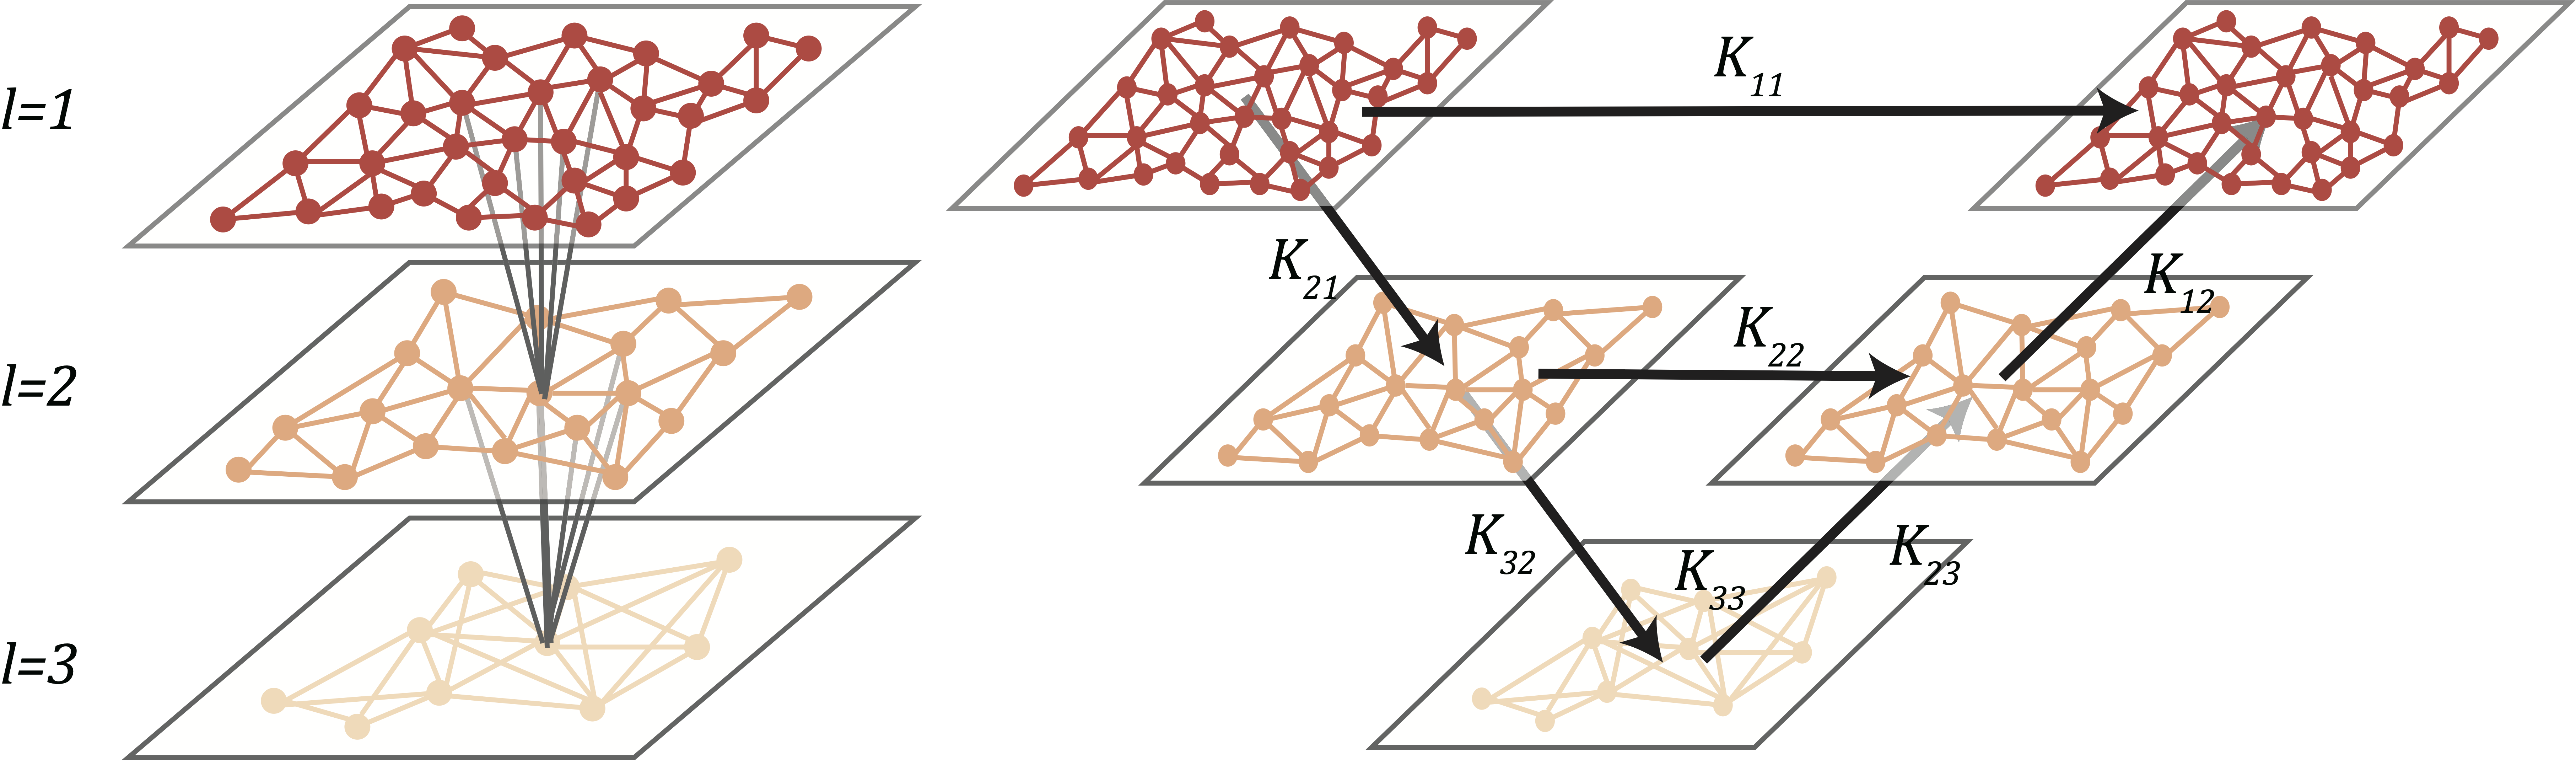
\includegraphics[width=\textwidth]{Figs/multigraph.png}
    \caption{V-cycle}\label{fig:vcycle}
    \label{fig:multigraph}
    \small{
    {\bf Left}: the multi-level discretization.  {\bf Right}: one V-cycle iteration for the multipole neural operator.
    }
    }
\end{figure}

\paragraph{V-cycle Algorithm}
We present a V-cycle algorithm, see Figure \ref{fig:vcycle}, for efficiently computing \eqref{eq:hierarchy_decomposition}. It consists of two steps: the \textit{downward pass} and the \textit{upward pass}. Denote the representation in downward pass and upward pass by $\vdown$ and $\vup$ respectively. In the downward step, the algorithm starts from the fine discretization representation $\vdown_1$ and updates it by applying a downward transition 
$\vdown_{l+1} = K_{l+1,l} \vdown_{l}$.
In the upward step, the algorithm starts from the coarse presentation $\vup_{L}$ and updates it by applying an upward transition and the center kernel matrix
$\vup_{l} = K_{l,l-1} \vup_{l-1} + K_{l,l} \vdown_l$. Notice that 
applying one level downward and upward exactly computes $K_{1,1} + K_{1,2}K_{2,2}K_{2,1}$, and a full $L$-level V-cycle leads to the multi-resolution decomposition \eqref{eq:hierarchy_decomposition}.

Employing \eqref{eq:all1}-\eqref{eq:all3}, we use $L$ neural networks $\kappa_{1,1}, \ldots, \kappa_{L,L}$ to approximate the kernel operators associated to $K_{l,l}$, and $2(L-1)$  neural networks $\kappa_{1,2}, \kappa_{2,1}, \dots$ to approximate the transitions  $K_{l+1,l}, K_{l,l+1}$.
Following the iterative architecture \eqref{eq:F}, we introduce the linear operator \(W \in \R^{n \times n}\)
(denoting it by \(W_l\) for each corresponding resolution) to help regularize the iteration, as well as the nonlinear activation function $\sigma$ to increase the expensiveness. \done{Previous sentence ends without making sense.} Since $W$ acts pointwise (requiring $J$ remains the same for input and output), we employ it only along with the kernel \(K_{l,l}\) and not the transitions. At each layer \(t=0,\dots,T-1\), we perform a full V-cycle as:

\begin{itemize}
    \item  Downward Pass
    \begin{equation}\label{eq:up}
    \textnormal{For}\ l = 1, \ldots, L: 
    \hspace{0.7in}
         \vdown_{l+1}^{(t+1)} = \sigma(\vup_{l+1}^{(t)} +  K_{l+1,l} \vdown_{l}^{(t+1)} )
     \hspace{1.3in}
    \end{equation}
    \item  Upward Pass
    \begin{equation}\label{eq:down}
    \textnormal{For}\ l = L, \ldots, 1: 
    \hspace{0.7in}
       \vup_{l}^{(t+1)} = \sigma( (W_l+ K_{l,l}) \vdown_{l}^{(t+1)}  +  K_{l,l-1} \vup_{l-1}^{(t+1)}).
   \hspace{0.5in}
    \end{equation}
\end{itemize}
Notice that one full pass of the V-cycle algorithm defines a mapping \(v \mapsto u\).

\paragraph{Multi-level Graphs.}
We emphasize that we view the discretization \(\{x_1,\dots,x_J\} \subset D\) as a graph in order to facilitate an efficient implementation through the message passing graph neural network architecture. Since the V-cycle algorithm works at different levels of the discretization, we build multi-level graphs to represent the coarser and finer discretizations. 
We present and utilize two constructions of multi-level graphs, the orthogonal multipole graph and the generalized random graph.
The orthogonal multipole graph is the standard grid construction used in the fast multiple method which is adapted to a uniform grid, see e.g. \citep{greengard1997new}. In this construction, the decomposition in \eqref{eq:decomposition_matrix} is orthogonal in that the finest graph only captures the closest range interaction, the second finest graph captures the second closest interaction minus the part already captured in the previous graph and so on, recursively. In particular, the ranges of interaction for each kernel do not overlap. While this construction is usually efficient, it is limited to uniform grids which may be a bottleneck for certain applications.
Our second construction is the generalized random graph as shown in Figure \ref{fig:hmatrix} where the ranges of the kernels are allowed to overlap. The generalized random graph is very flexible as it can be applied on any domain geometry and discretization. Further it can also be combined with random sampling methods to work on problems where \(J\) is very large or combined with an active learning method to adaptively choose the regions where a finer discretization is needed. 

\paragraph{Linear Complexity.}
Each term in the decomposition \eqref{eq:decomposition_matrix} is represented by the kernel matrix   \(K_{l,l}\) for $l = 1,\ldots, L $, and \(K_{l+1,l}, K_{l,l+1}\) for $l = 1, \ldots, L-1 $ corresponding to the appropriate sub-discretization.
Therefore the complexity of the multipole method is 
 $\sum_{l=1}^L \mathcal{O}(J^2_l r_l^d) + \sum_{l=1}^{L-1}\mathcal{O}(J_l J_{l+1} r_l^d) = \sum_{l=1}^L \mathcal{O}(J^2_l r_l^d)$.
By designing the sub-discretization so that $\mathcal{O}(J^2_l r_l^d) \leq \mathcal{O}(J)$, we can obtain  complexity linear in $J$. 
For example, when $d=2$, pick \(r_l = 1/\sqrt{J_l}\) and \(J_l = \mathcal{O}(2^{-l} J)\) such that \(r_L\) is large enough so that there exists a ball of radius \(r_L\) containing \(D\). Then clearly $\sum_{l=1}^L \mathcal{O}(J^2_l r_l^d) = \mathcal{O}(J)$. 
By combining with a Nystr\"om approximation, we can obtain $\mathcal{O}(J')$ complexity for some \(J' \ll J\).
